\documentclass[12pt,fleqn]{exam}
\usepackage{pifont}
\usepackage{dingbat}
\usepackage{amsmath,amssymb}
\usepackage{epsfig}
\usepackage[colorlinks=true,linkcolor=black,anchorcolor=black,citecolor=black,filecolor=black,menucolor=black,runcolor=black,urlcolor=black]{hyperref}
\usepackage[letterpaper, margin=0.75in]{geometry}
\usepackage{tikz}
\usetikzlibrary{arrows}
\addpoints
\boxedpoints
\pointsinmargin
\pointname{pts}

\usepackage{pdfpages}
\usepackage[final]{microtype}
\usepackage[american]{babel}
\usepackage[T1]{fontenc}
\usepackage{fourier}
\usepackage{isomath}
\usepackage{upgreek,amsmath}
\usepackage{amssymb}

\newcommand{\dotprod}{\, {\scriptzcriptztyle
    \stackrel{\bullet}{{}}}\,}

\newcommand{\reals}{\mathbf{R}}
\newcommand{\lub}{\mathrm{lub}} 
\newcommand{\glb}{\mathrm{glb}} 
\newcommand{\complex}{\mathbf{C}}
\newcommand{\dom}{\mbox{dom}}
\newcommand{\range}{\mbox{range}}
\newcommand{\cover}{{\mathcal C}}
\newcommand{\integers}{\mathbf{Z}}
\newcommand{\degree}{\mathrm{degree}}
\newcommand{\vi}{\, \mathbf{i}}
\newcommand{\vj}{\, \mathbf{j}}
\newcommand{\vk}{\, \mathbf{k}}
\newcommand{\bi}{\, \mathbf{i}}
\newcommand{\bj}{\, \mathbf{j}}
\newcommand{\bk}{\, \mathbf{k}}
\newcommand{\dist}{\, \mathrm{dist}}
\DeclareMathOperator{\Arg}{\mathrm{Arg}}
\DeclareMathOperator{\Ln}{\mathrm{Ln}}
\newcommand{\imag}{\, \mathrm{i}}

\usepackage{xcolor}
\shadedsolutions
\definecolor{SolutionColor}{rgb}{0.95,0.95,0.95}

\usepackage{graphicx}
\newcommand\AM{{\sc am}}
\newcommand\PM{{\sc pm}}
     
%\usepackage{twemojis}
\newcommand{\quiz}{8}
\newcommand{\term}{Spring}
\newcommand{\due}{9:55 \AM}
\newcommand{\class}{MATH 102}
\begin{document}
\large
\vspace{0.1in}
\noindent\makebox[3.0truein][l]{\textbf{\class, \term \/ \the\year}}
\textbf{Name:} \hrulefill \\
\noindent \makebox[3.0truein][l]{\textbf{In class work \quiz}}
\textbf{Row and Seat}:\hrulefill\\
\vspace{0.1in}

\begin{quote}
``\emph{The place to improve the world is first in one's own heart and head 
and hands, and then work outward from there.} \hfill {\sc Robert M. Pirsig}
\end{quote}
\noindent  In class work  \quiz\/  has questions 1 through  \numquestions \/ with a total of  \numpoints\/  points.   
 This assignment is due at the end of the class period (\due).
This assignment is printed on \textbf{both} sides of the paper.
\vspace{0.1in}


\begin{questions} 

 \question For the polynomial $P(x) = \frac{1}{50} (x+4)(x-6)^2$, do the following:

 \begin{parts}

    \part [2] Find $\degree(P)$.
    \begin{solution}[0.5in]
    \end{solution}
        
    \part [2] Find the x-intercepts of the equation $y = P(x)$.
    \begin{solution}[0.75in]
    \end{solution}

    \part[2] At each x-intercept, determine if $P$ is increasing or decreasing.
    To do this, follow the process we learned in class and fill out the chart. 
    To help you start, I did one row for you.

    \vspace{0.5in}
    \large
    \begin{tabular}{|c|c|c|} \hline 
      Zero  & $P(x) \approx $ & increasing or decreasing  \\ \hline 
      $-4$  & $2 (x+4)$ &   increasing \\ \hline
      $  $  & $       $ &               \\ \hline 
    \end{tabular}
    \normalsize
    \part[2] Draw a PGG (pretty good graph) of $P$

    \vfill

  \end{parts}

\newpage

\question Shown below is a graph of a polynomial $W$.  Several points on
the graph are labeled. (The point labeled $(0.5, 2.531)$ is actually the point 
$(0.5, 2.53125)$.)  Given that the $\degree(W)=4$, find a formula for $W$.

\begin{figure*}[h]
    \begin{center}

    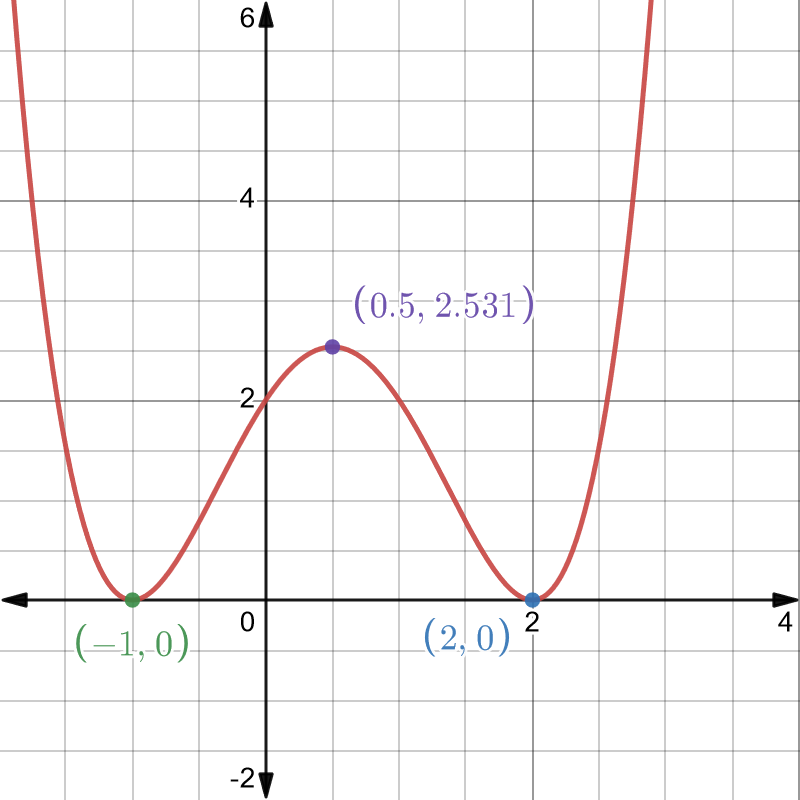
\includegraphics[scale=0.25]{desmos-graph(40).png}
    \end{center}

\end{figure*}

\end{questions}
\end{document}
